%%% fs-state-model - Model

\label {fs-model-section}

In this section we outline the model of our system. We focus on the core concepts and definitions in order to introduce the necessary preliminaries for consistency preserving mechanisms.

\subsection{Data flow}
The basic data flow abstraction is a {\it stream}. The stream is represented by an infinite heterogeneous sequence of data items. Data item is a {\it payload} and a {\it meta-information} associated with it. 

\[DataItem := (Payload, Meta)\]

The payload is an arbitrary user-provided data. Meta is structured system-assigned information. The primary purpose of the meta-information is to impose the total order on data items. 

Data payloads are generated by data producers and are got into the stream through {\it front}. They got out of the stream to data consumers through {\it barrier}. Front creates data items from input events by assigning them meta-information. Inside stream, data items can be dropped or their payloads and metas can be transformed. Barrier removes meta-information and outputs back pure payloads. 

\subsection{Computational flow}
The stream between front and barrier is handled by a directed data flow graph. Each node of the graph represents a single operation, which can have multiple inputs and outputs. Edges indicate the order of these operations. Data items are processed one-by-one in a "streaming" manner. Our model allows cycles in the graph while data flow graphs are commonly assumed to be acyclic (DAGs) 
~\cite{Zaharia:2016:ASU:3013530.2934664, Carbone:2017:SMA:3137765.3137777}.

\subsection{Physical deployment and partitioning}
Data flow graph is distributed among computational units. Each unit runs a process called {\it worker}, and each of the workers executes complete data flow graph. The range of 32-bit signed integer is divided into the fixed number of non-intersecting {\it hash units}. Each worker can be responsible for one or many hash units. Hash units are used further for partitioning and state saving. The number of hash-units per worker is a user-defined parameter and it must be set before the start of computations. 

Each operation input has a user-provided hash function called {\it balancing function}. This function is applied to the payload of data items and determines partitioning before each operation. After that, the data items are sent to the worker, which is responsible for the associated hash unit. Therefore, load balancing explicitly depends on the user-defined balancing functions. This allows the developer to determine optimal balancing which requires the knowledge of the payload distribution. The system optimizes the hash ranges assignment according to the processing statistics. 

\subsection{Ordering assumptions}
We assume that there is a total order on data items. Ordering is preserved when an item is going through the operations. More precisely, the order of output items is the same as the order of corresponding input items. If more than one item is generated, they are inserted in output stream sequentially. Moreover, the output follows corresponding input but precedes the next item. Without diving into details, it should be noted that the order of items is maintained across different fronts.

The concept of ordering is shown in Figure~\ref{ordering}. Data item with payload $1'$ is the derivative of the item with payload $1$, according to operation $F$. The same is for items with payloads $2'$ and $2$. After union operation, the order between $1$ and $2$ is preserved. Furthermore, $1'$ follows $1$, and $2'$ follows $2$.  
\begin{figure}[htbp]
  \centering
  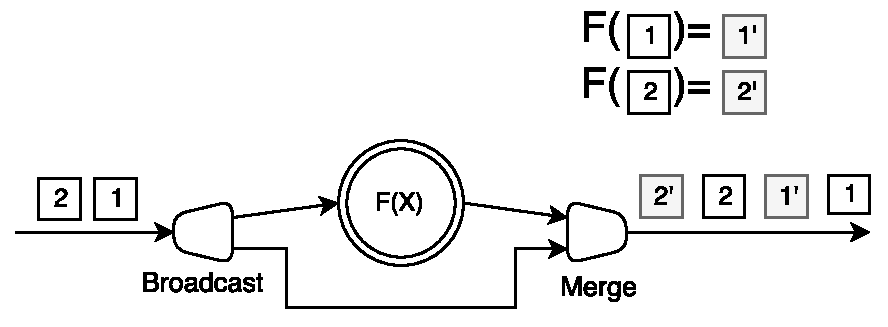
\includegraphics[width=0.5\textwidth]{pics/ordering}
  \caption{The concept of ordering model}
  \label {ordering}
\end{figure}

We assume that input items of the operations are strictly ordered.

\subsection{Supported operations}
The list of available operations includes:

{\bf Map} applies a user-defined function to the payload of an input item. This function returns a sequence of data items with transformed payloads. An output sequence can be empty.

{\bf Broadcast} replicates an input item to the specified number of operations.

{\bf Merge} operation is initialized with the specified number of input nodes. It sends all incoming data to the output.

{\bf Grouping} has a {\it window size} parameter. Grouping stores input items into distinct buckets by the value of the input balancing function applied to the payload. When the next item arrives at the grouping, it is appended to the corresponding bucket. Each time the grouping outputs window-sized {\it tuple item}, which consists of the most recent (in terms of the meta-information) items of this bucket. If the size of the bucket is less than the window, all items of the bucket are taken. Grouping is the only operation that has a state.

The following example illustrates the semantics of the operation. The grouping accepts items with payload represented as natural numbers: 1,2,3, etc. The hash function returns 1 if the number is even and 0 otherwise. If the window is set to 3, the output is:

\[(1), (2), (1|3), (2|4), (1|3|5), (2|4|6), (3|5|7), (4|6|8)...\]

There are two important properties of the grouping operation: the output tuple is identified by its last element, the results among items with different values of a hash function are independent.

\subsection{Stateful transformations}
The given set of operations jointly with cyclic execution graphs is enough to implement any stateful operation, i.e. reduce in terms of MapReduce model. The scheme of such transformations is out of scope within this paper, however, it is deeply detailed in~\cite{we2018seim}.

\subsection{Consistency guarantees}
There are three main types of consistency guarantees relating to stream processing. {\it At most once} semantics states that each input event is processed once or not processed at all. {\it At least once} guarantees that each input item is processed, but possibly multiple times, that can lead to result duplication. {\it Exactly once} semantics guarantee that each input event is processed exactly one time. The techniques to achieve these guarantees in the presence of failures are detailed in the next section.

\subsection{Implementation notes}

As it was defined previously, only the grouping operation maintains a state and the state depends on the order of incoming items. Therefore, there is a need to enforce the right order to achieve deterministic processing. However, conservative methods for the order enforcing are based on buffering~\cite{Li:2008:OPN:1453856.1453890} and can imply high latency overhead. The main difficulty here is that items can be easily reordered within stream processing systems because of asynchrony and the possible existence of multiple paths between two nodes. 

In~\cite{we2018seim} we proposed an optimistic approach to handle out-of-order items. The key idea behind it is that grouping can produce invalid results, but they must be filtered out at the barrier. Therefore, there is a need to buffer output items at the barrier before it is ensured that there are no in-flight invalid items and the cannot be generated. In order to minimize latency, it is convenient to release items by global times.

To track the global time of in-flight items we adopt an idea of {\it acker task} inspired by Apache Storm~\cite{apache:storm}. Acker tracks data items using a checksum hash. When the item is sent or received by an operation, its global time and checksum are sent to the acker. This message is called {\it ack}. Acker groups acks by a global time into the structure called {\it ack table}. Once acker receives an ack message with global time {\it GT} and {\it XOR} it updates {\it GT} entry in the table by xoring {\it XOR} with the current value. When an item is sent and later received by the next operation, xoring corresponding {\it XOR}s would yield zero.

Acks are overlapped to nullify table's entry only when an item arrives at the barrier. That is, ack for receive is sent only after both processing and the ack sending for the transformed item, as illustrated in Figure~\ref{acker}. Different shapes of items mean different payloads. The ack for the sending of the triangular element is sent before the rectangular one. We expect the channel between the acker and each operation to be FIFO, so ack for the triangular item would be xored before the rectangular. So the two equal values are separated by distinct one. 

This technique guarantees that the {\it XOR} for some global time is equal to zero only if there are no in-flight elements with such global time.

\begin{figure}[htbp]
  \centering
  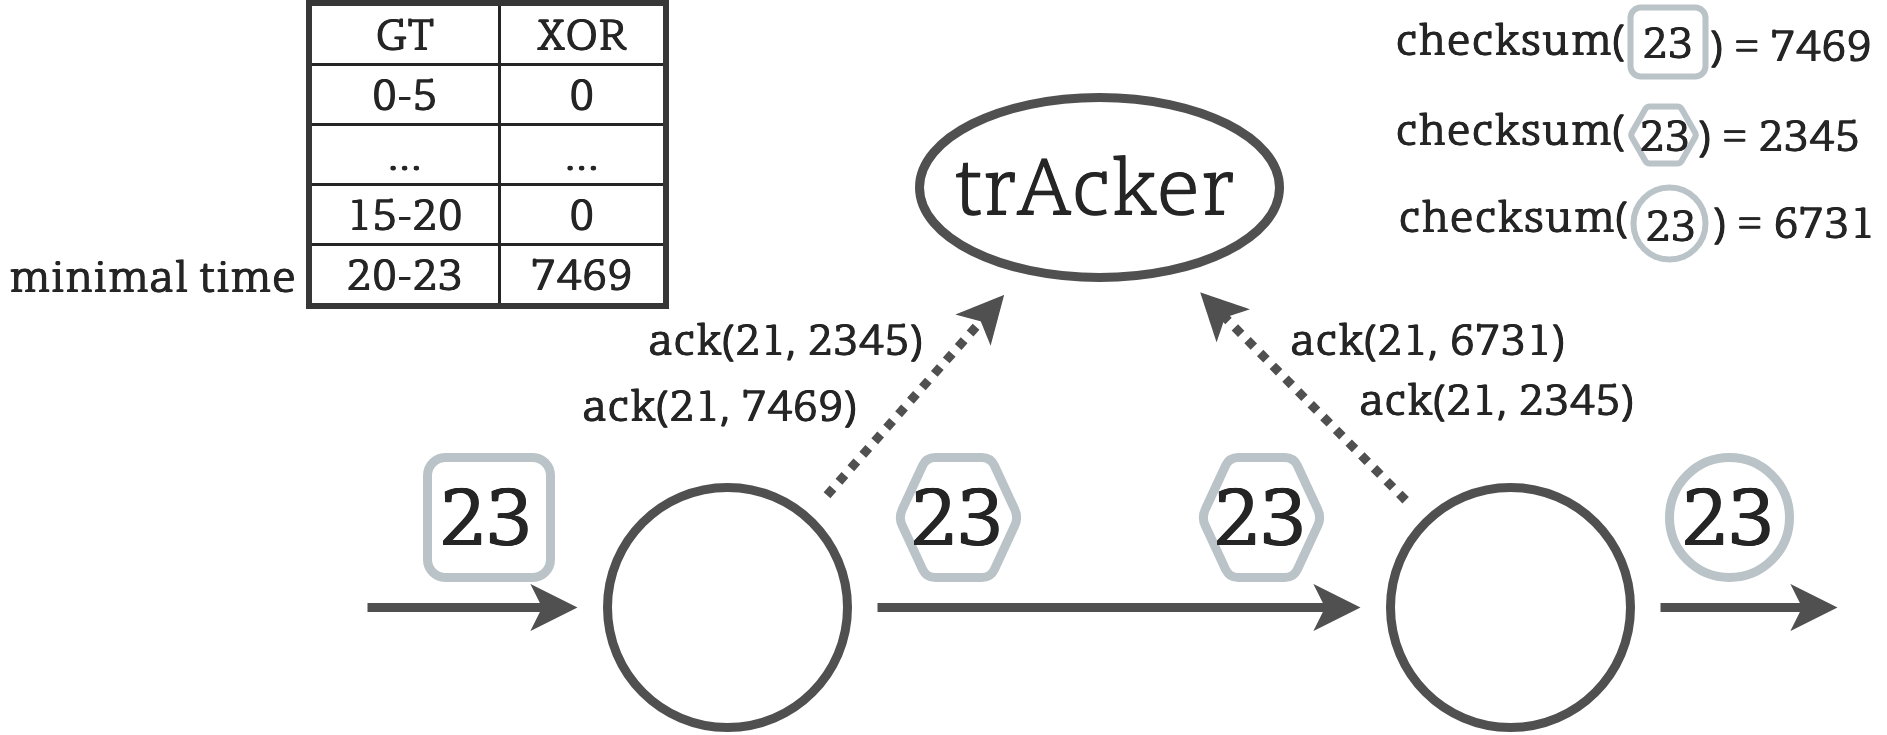
\includegraphics[scale=0.6]{pics/acker}
  \caption{The example of tracking minimal time using acker}
  \label {acker}
\end{figure}

The minimal time within a stream is the minimal global time with non-zero {\it XOR}. On minimal time changes, acker broadcasts new minimal time to the barrier and operations. Therefore, the barrier can release elements with global time {\it GT} once it received notification from acker that the minimal time within the stream is greater than {\it GT}.

To ensure that no fronts can generate item with the specific timestamp, each front periodically sends to acker special message called {\it report}, which promises that front will not generate items with a timestamp lower than the reported. The value in the ack table can become zero only after the corresponding report arrives.

It must be noted that acker can play the role of worker's coordinator because it observes the progress of the whole system. This property is used further in the implementation of mechanisms for fault tolerance. 

\FlameStream\ is implemented in Java, using Akka framework for messaging and applies Apache ZooKeeper as a {\it cluster state manager}. The usage of ZooKeeper mitigates the need for the dedicated master node. An overview of the \FlameStream\ system model and architecture is shown in Figure[NEED FOR PIC].
